\chapter{Introduction}
\label{chap:Introduction}

The widespread adoption of the internet in modern culture has caused a large evolution in the way we use computers.
When computers were still new almost all programs and services were run locally on the machine.
Nowadays our usage has shifted to a multitude of online services and solutions.
One of the more well known examples is digital encyclopedias: Microsoft Encarta was distributed on a single CD upon release.
But today Wikipedia has become synonymous with looking up information --  a large encyclopedia service which can be accessed via the internet.
Other examples can be found a plenty: almost anything is available as a cloud service, from games to web hosting.

Therefore it should come as no surprise that storing data has also increasingly shown trends to moving onto the internet.
And indeed the multitude of online data storage services in existence today show the rising trend to store data -- not on personal machines -- but to entrust it to third party service providers.
Such third party services provide users with access to their data wherever they can access the internet in general.
Dropbox~\cite{web:site:dropbox} made its name as a popular data storage service provider, but existing internet giants were quick to follow.
Thus both Google and Microsoft also began offering competing services: Google Drive~\cite{web:site:gdrive} and OneDrive~\cite{web:site:onedrive} respectively.

All was well for a while.
Users merrily entrusted their data to third parties under the reasoning of ease of access and ease of use.
Private data would no longer be lost if the personal computer stopped functioning for one reason or the other.
Additionally the rise of mobile devices such as smartphones only quickened the adoption of cloud storage services.
The exorbitant pricing of storage space and the lack of removable external storage on these mobile devices drove people to solutions that allowed them to access all their data nonetheless.

In 2013 Edward Snowden revealed that the blind trust in these third party services was misplaced.
Thanks to Snowden's whistle blowing and personal sacrifice a global conspiracy of governmental agencies that undertake massive online surveillance of most internet communications was brought to the public attention.
Since the majority of the global internet players are based in the United States of America, this had huge implications for all services offered via the internet.
Many services used by the majority of internet users have been shown to be either at risk of being or already are compromised or even known to explicitly include capabilities for compromising data security.
This includes internet giants such as Microsoft, Yahoo, Google, Facebook, Paltalk, AOL, Skype, YouTube, and Apple~\cite{web:site:wp:internet_giants}.
Snowden also revealed that most data passing through internet exchange points is surveilled~\cite{web:site:heise:decix}.
These form the backbone of the internet in its current state.

While public outrage lasted just as long as the major news outlets covered it, the revelations had a major impact in the technical community.
New software solutions were required to enable users to reconquer their privacy on the internet without sacrificing usability and ease of access.
One example is the Open Whisper Systems group.
Their stated goal on the website is "[...] we're working to advance the state of the art for secure communication, while simultaneously making it easy for everyone to use."~\cite{web:site:whispersystems}.
Another example is the Tox instant messenger community that is building a free, open source, peer to peer Skype alternative~\cite{web:site:tox}.

\section{Motivation}
\label{sec:Motivation} %NOTE: this is linked against, don't remove

The thesis is mainly motivated by the revelations of drag net surveillance by Edward Snowden and the compliance of so called trusted service providers within their legal obligations and even beyond.
The uncovering of the global surveillance network has shown that we can not entrust third parties with our data without taking additional steps to secure it.
While services such as Boxcryptor~\cite{web:site:boxcryptor} exist to add a layer of encryption on top of the data storage services they bring with them a few disadvantages in terms of ease of use.
Notably for this specific example access to the encrypted data is severely hampered because it can not be accessed via the internet without first decrypting it additionally.

Services exist that do not rely on a user's trust to a third party.
These peer to peer solution promise to keep all data of the user only on the user's machines.
However the lack of a copy of the data on a remote server removes the advantages of web access over the internet and decrease their utility as data backup services.
Examples for existing peer to peer solutions include BitTorrent Sync~\cite{web:site:bittorrent_sync} and Syncthing~\cite{web:site:synthing}.

Our motivation stems from the hope that we can combine the two types of offering data storage services into one service that retains most of the advantages.
Thus we propose the implementation of a peer to peer, fully encrypted file synchronization system that is capable of storing encrypted backups of users' data on third party servers while still allowing remote access to it via the internet.
We therefore define two types of peers: trusted peers that store data unencrypted and are intended for the trusted devices of users and encrypted peers that remove the need to trust third parties while still allowing them to serve as remote storage providers.

\section{Goals}
\label{sec:Goals}

This work thus has the goal of designing and implementing a proof of concept that such a service is possible.
The proposed implementation should build on peer to peer communication, bypassing the requirement of a centrally hosted third party service.
Unlike most existing peer to peer solutions we propose to include support for encrypted third parties so that the advantages of remote storage are kept.
To harden such a peer to peer network it is necessary to encrypt all communication between the peers.
Instead of integrating and mixing encrypted communications with the file synchronization commands required for such software to work, we utilize an existing secure peer to peer communication infrastructure in the form of Tox, on top of which we will propose a protocol for the sole task of file synchronization.
The encryption scheme is to be chosen so that while encrypted peers are denied access to a user's data, authorized access over the internet is still possible.
To facilitate a high flexibility of the encrypted peer we will also work to implement a storage interface that allows any desired storage system to be used with a user's data, from direct disk storage to distributed file systems.

The implementation of the program will be done with Golang, building on Tox for the communication and the Hadoop distributed file system for storing data on the encrypted peer.
We will expand on the specification and define the scope of this work in preparation.
Apart from the theoretical work a large part of this thesis is also the implementation of a proof of concept.
Therefore we will also discuss problems we encountered while working on the software aspect and our solutions to them.
Finally we will look back at the implementation and compare it to the theoretical ground work.
For a better comparison a brief discussion on similarities and differences to existing file synchronization services will also be included.

\section{Name}
\label{sec:Name}

\begin{figure}[htp]
\centering
    
\includegraphics[width=1.5cm]{img/icon}
\caption[Tinzenite Icon]{The preliminary icon of our implementation of Tinzenite.}
\label{fig:icon}
\end{figure}

To differentiate our proof of concept implementation from existing solutions a unique name was required.
We chose the rock-forming mineral tinzenite for the name.
We wanted a name that had some association to a crystal to signify the hardened security aspect of our work.
Furthermore the crystal has a unique orange color that lends itself well as an icon as can be seen in figure~\ref{fig:icon}.
Specifically, Tinzenite is the name of the peer network which in turn is compromised of two distinct software peers which are based on a common protocol and communication standard.

\section{Structure}
\label{sec:Structure}

\begin{figure}[htp]
\centering
    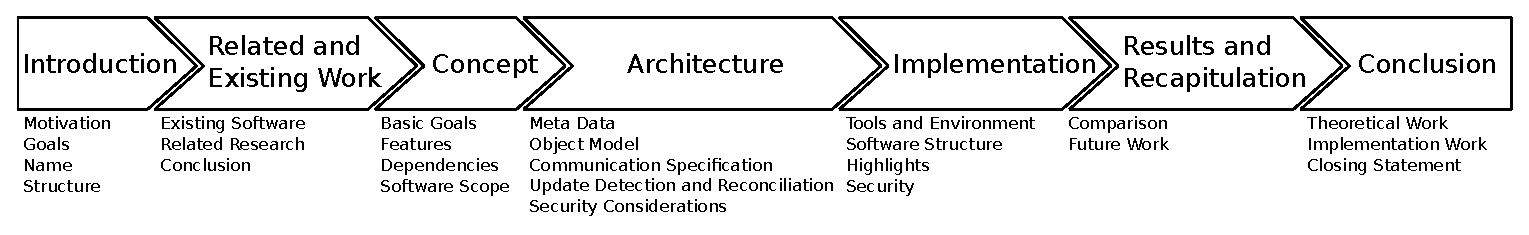
\includegraphics[width=\linewidth]{diagram/thesis_structure}
\caption[Thesis Structure Diagram]{A graphical representation of the structure of this thesis.}
\label{fig:thesis_structure}
\end{figure}

Chapter~\ref{chap:Related and Existing Work} presents existing software that is relevant to our work, as well as related papers.
Built on this we will define the concept of this thesis in chapter~\ref{chap:concept}.
Chapter~\ref{chap:architecture} describes the theoretical architecture that Tinzenite will be based on.
The implementation of the architecture into our proof of concept implementation will be discussed in chapter~\ref{chap:Implementation}.
We will expand on the completed work in chapter~\ref{chap:Results and Recapitulation} and note what possible future work could be built on top of the provided thesis.
Finally chapter~\ref{chap:conclusion} will conclude this thesis and provide a general closing statement.
Figure~\ref{fig:thesis_structure} shows a graphical representation of the structure of this thesis.
